\part{Transformers}
\title{Transformers}  
\date{}  
\frame{\titlepage} 

%%%%%%%%%%%%%%%%%%%%%%%%%%%%%%%%%%%%%%%%%%%%%%%%%%%%%%%%%%%%%
%% Transformer definition %%
%%%%%%%%%%%%%%%%%%%%%%%%%%%%%%%%%%%%%%%%%%%%%%%%%%%%%%%%%%%%%
\begin{frame}
	\frametitle{Transformer definition}
    \begin{columns}
		\begin{column}{0.65\textwidth}
            \begin{varblock}{Transformer}
                A transformer is a static device that transfers electrical energy between two or more circuits through electromagnetic induction. It converts the AC voltage levels between inputs and outputs.   
            \end{varblock}
            \begin{itemize}
                \item While a transformer is sometimes called a ``static~machine'', it does not meet the formal definition of an electrical machine (compare first chapter).
                \item However, transformers share some working principles with electrical machines and are also often used as components of electrical power systems including drives.
            \end{itemize}
		\end{column}
        \hfill
		\begin{column}{0.35\textwidth}
			\begin{figure}
				\centering
				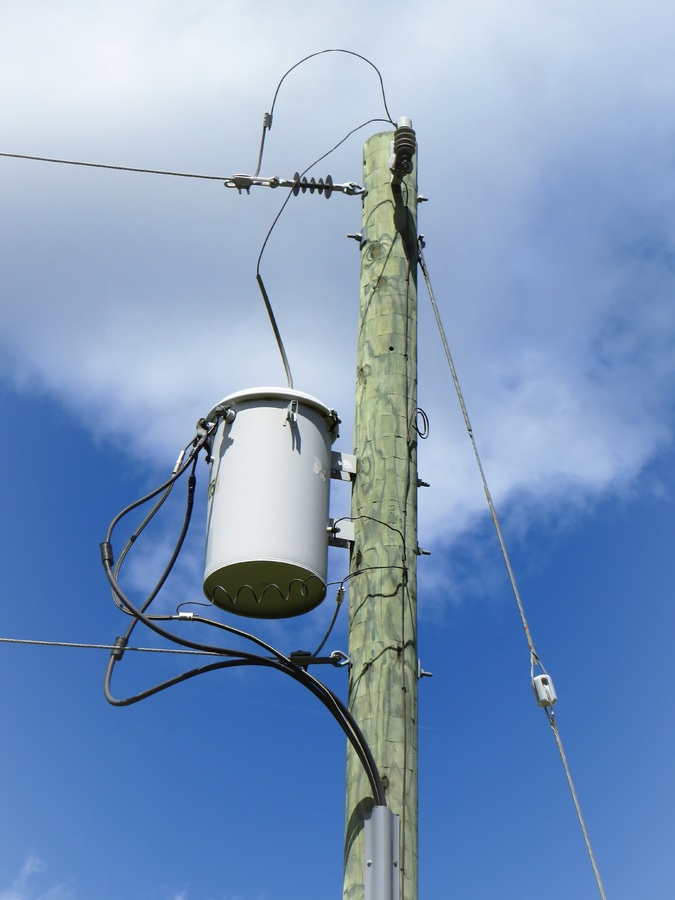
\includegraphics[width=0.75\textwidth]{fig/lec04/Transformer_rural_pole.jpg}
				\caption{Transformer integrated at a utility pole (source: \href{https://pxhere.com/en/photo/795672}{pxhere.com}, public domain)}
			\end{figure}
		\end{column}
		\end{columns}
\end{frame}

%%%%%%%%%%%%%%%%%%%%%%%%%%%%%%%%%%%%%%%%%%%%%%%%%%%%%%%%%%%%%
%% Examples of transformers %%
%%%%%%%%%%%%%%%%%%%%%%%%%%%%%%%%%%%%%%%%%%%%%%%%%%%%%%%%%%%%%
\begin{frame}
	\frametitle{Examples of transformers}
	\begin{figure}
		\centering
		\begin{subfigure}[b]{0.49\textwidth}
			\centering
			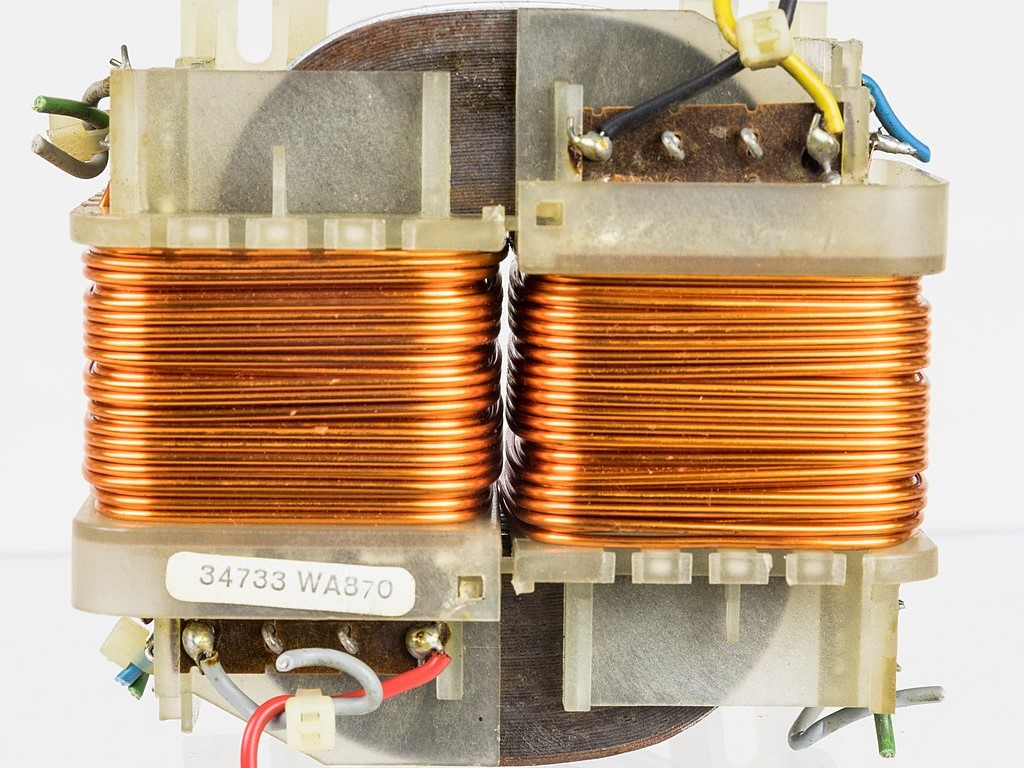
\includegraphics[width=0.45\textwidth]{fig/lec04/Power_supply_transformer.jpg}
			\caption{Power supply transformer (source: \href{https://commons.wikimedia.org/wiki/File:Philips_N4422_-_power_supply_transformer-2098.jpg}{Wikimedia Commons}, R.~Spekking, \href{https://creativecommons.org/licenses/by-sa/4.0/deed}{CC BY-SA 4.0})}
		\end{subfigure}
		\hfill
		\begin{subfigure}[b]{0.49\textwidth}
			\centering
			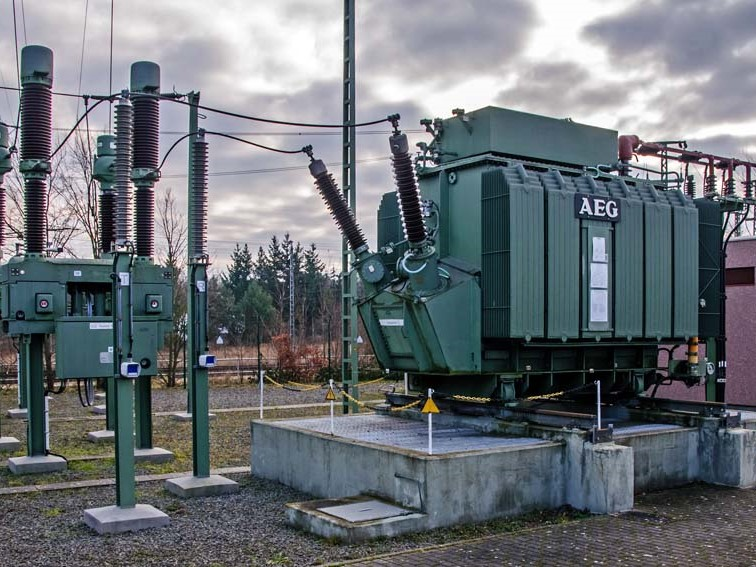
\includegraphics[width=0.45\textwidth]{fig/lec04/Single_phase_transformer.jpg}
			\caption{Single-phase transformer (source: \href{https://commons.wikimedia.org/wiki/File:DB_Unterwerk_Güsen,_Trafo_p.jpg}{Wikimedia Commons}, Georg, \href{https://creativecommons.org/licenses/by-sa/4.0/deed.en}{CC BY-SA 4.0})}
		\end{subfigure}
		\\
		\begin{subfigure}[b]{0.49\textwidth}
			\centering
			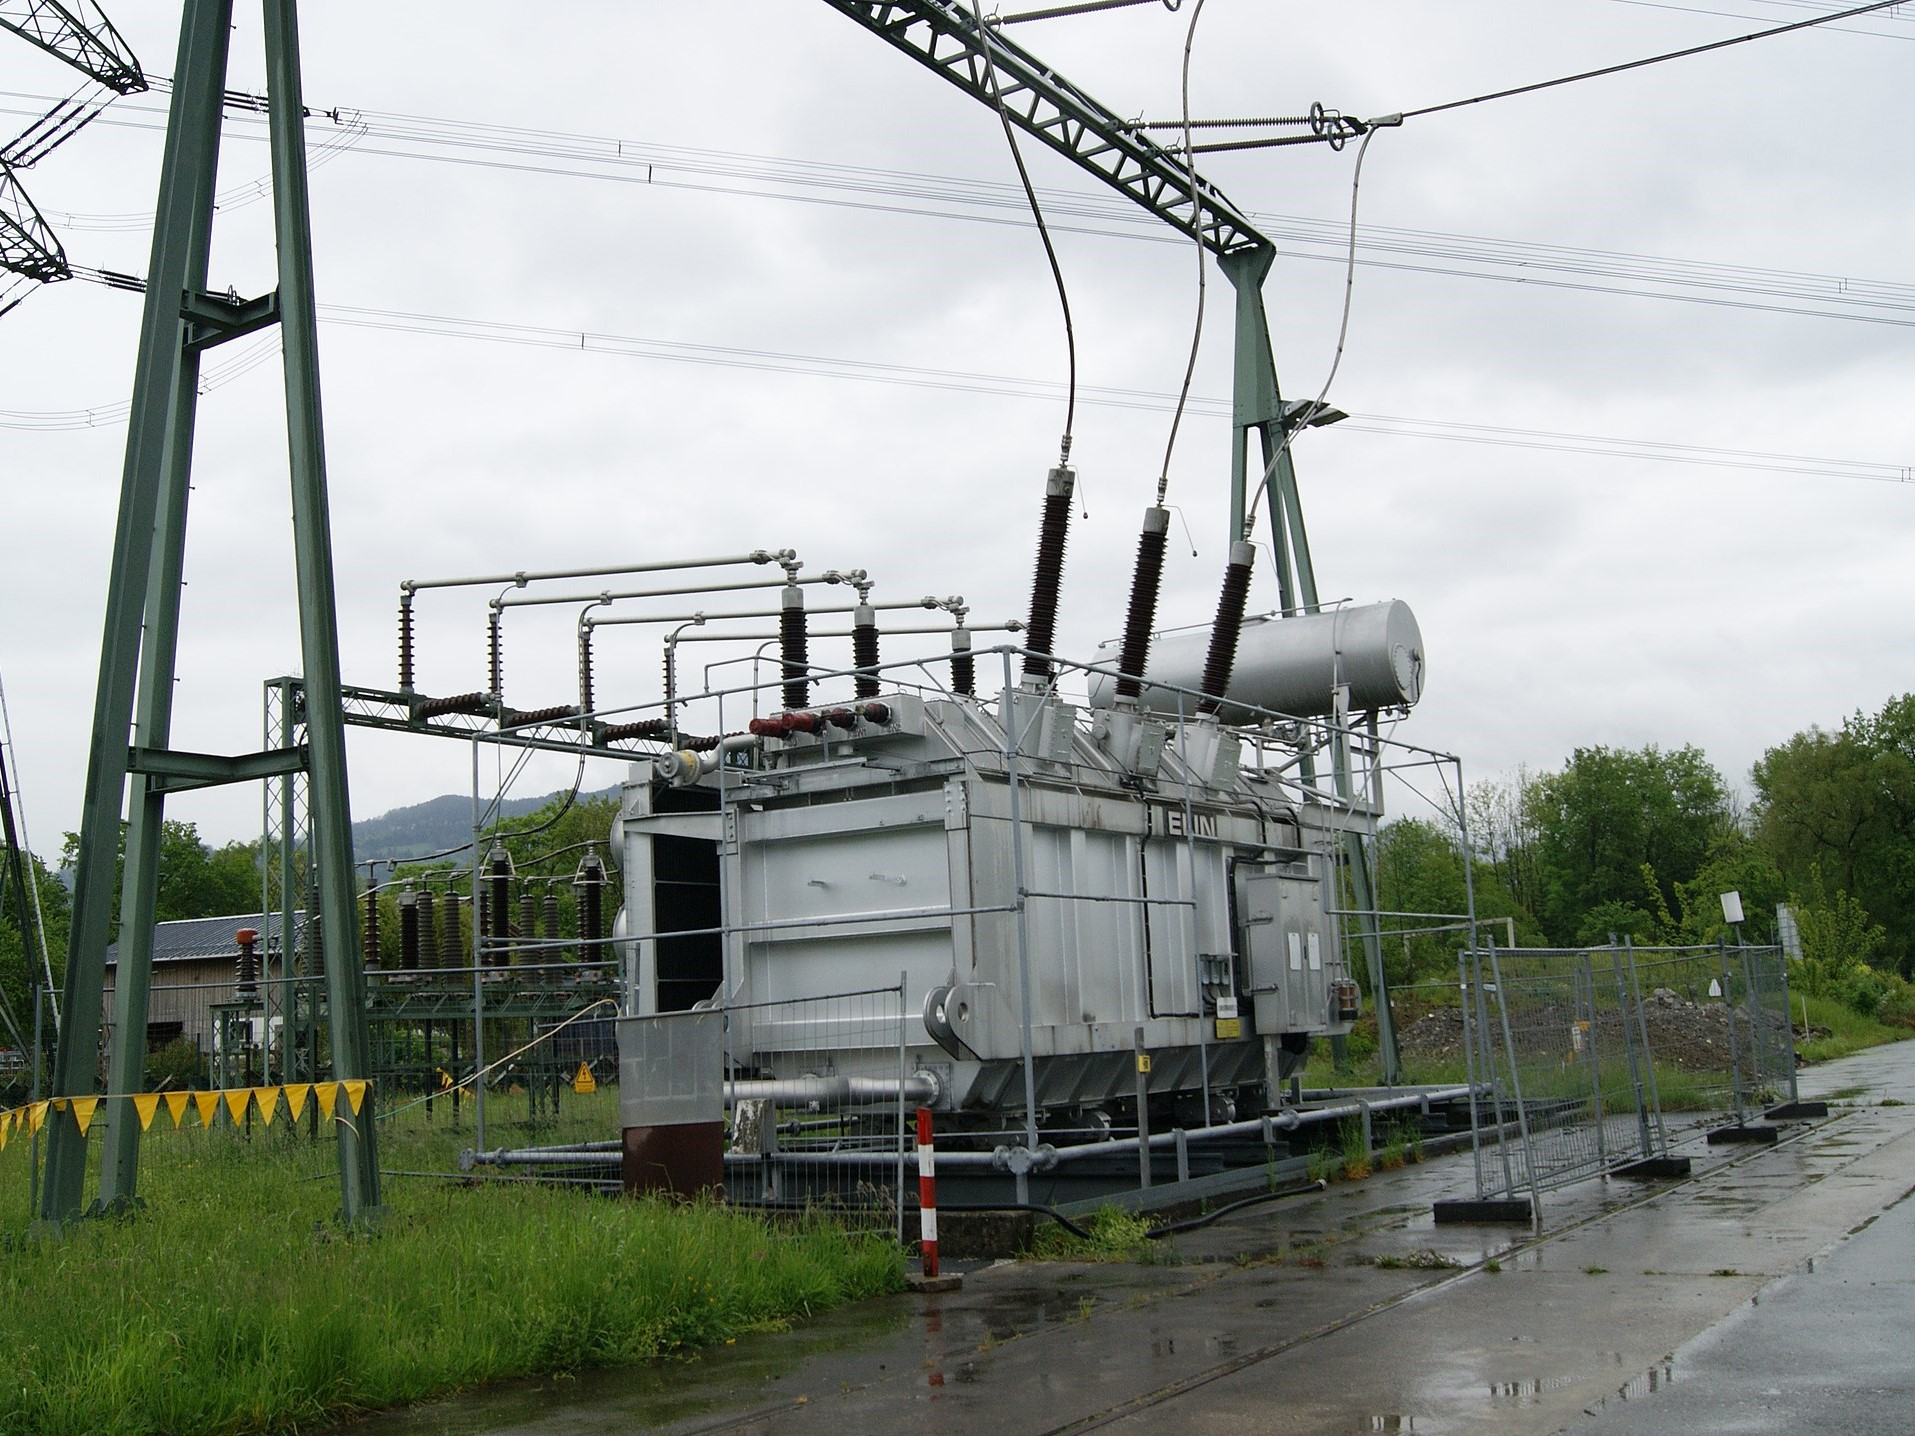
\includegraphics[width=0.45\textwidth]{fig/lec04/Three_phase_transformer.jpg}
			\caption{Three-phase transformer (source: \href{https://commons.wikimedia.org/wiki/File:Dornbirn-Umspannwerk_Werben-110kV_FS6-Anlage_Trafo_Elin_220-110kV-01ASD.jpg}{Wikimedia Commons}, Asurnipal, \href{https://creativecommons.org/licenses/by-sa/4.0/deed.en}{CC BY-SA 4.0})}
		\end{subfigure}
		\hfill
		\begin{subfigure}[b]{0.49\textwidth}
			\centering
			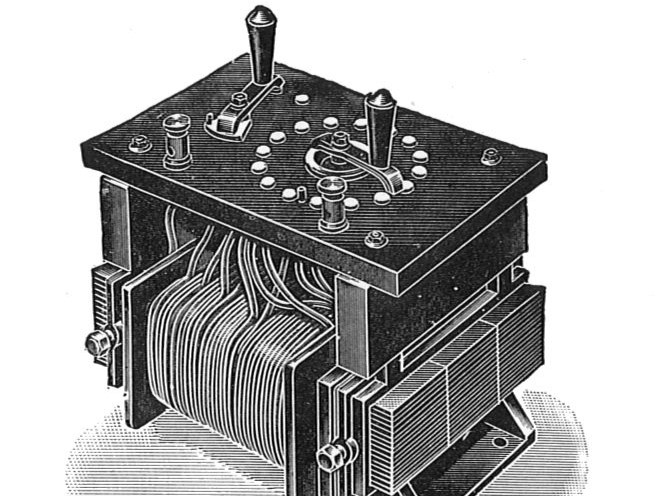
\includegraphics[width=0.45\textwidth]{fig/lec04/Tapped_transformer.jpg}
			\caption{Variable tapped transformer (source: \href{https://commons.wikimedia.org/wiki/File:Variable-tap_regulating_transformer_(Rankin_Kennedy,_Electrical_Installations,_Vol_II,_1909).jpg}{Wikimedia Commons}, public domain)}
		\end{subfigure}
		\caption*{Examples of transformers} 
        \label{fig:examples_transformers}
	\end{figure}
\end{frame}